%package list
\documentclass{article}
\usepackage[top=3cm, bottom=3cm, outer=3cm, inner=3cm]{geometry}
\usepackage{multicol}
\usepackage{graphicx}
\usepackage{url}
%\usepackage{cite}
\usepackage{hyperref}
\usepackage{array}
%\usepackage{multicol}
\newcolumntype{x}[1]{>{\centering\arraybackslash\hspace{0pt}}p{#1}}
\usepackage{natbib}
\usepackage{pdfpages}
\usepackage{multirow}
\usepackage[normalem]{ulem}
\useunder{\uline}{\ul}{}
\usepackage{svg}
\usepackage{xcolor}
\usepackage{listings}
\lstdefinestyle{ascii-tree}{
    literate={├}{|}1 {─}{--}1 {└}{+}1 
  }
\lstset{basicstyle=\ttfamily,
  showstringspaces=false,
  commentstyle=\color{red},
  keywordstyle=\color{blue}
}
%\usepackage{booktabs}
\usepackage{caption}
\usepackage{subcaption}
\usepackage{float}
\usepackage{array}

\newcolumntype{M}[1]{>{\centering\arraybackslash}m{#1}}
\newcolumntype{N}{@{}m{0pt}@{}}


%%%%%%%%%%%%%%%%%%%%%%%%%%%%%%%%%%%%%%%%%%%%%%%%%%%%%%%%%%%%%%%%%%%%%%%%%%%%
%%%%%%%%%%%%%%%%%%%%%%%%%%%%%%%%%%%%%%%%%%%%%%%%%%%%%%%%%%%%%%%%%%%%%%%%%%%%
\newcommand{\itemEmail}{vmamanian@unsa.edu.pe}
\newcommand{\itemStudent}{Victor Mamani Anahua}
\newcommand{\itemCourse}{Fundamentos de la Programación II}
\newcommand{\itemCourseCode}{20230489}
\newcommand{\itemSemester}{II}
\newcommand{\itemUniversity}{Universidad Nacional de San Agustín de Arequipa}
\newcommand{\itemFaculty}{Facultad de Ingeniería de Producción y Servicios}
\newcommand{\itemDepartment}{Departamento Académico de Ingeniería de Sistemas e Informática}
\newcommand{\itemSchool}{Escuela Profesional de Ingeniería de Sistemas}
\newcommand{\itemAcademic}{2023 - B}
\newcommand{\itemInput}{Del 08 Diciembre 2024}
\newcommand{\itemOutput}{Al 15 Diciembre 2024}
\newcommand{\itemPracticeNumber}{20}
\newcommand{\itemTheme}{Laboratorio 20}
%%%%%%%%%%%%%%%%%%%%%%%%%%%%%%%%%%%%%%%%%%%%%%%%%%%%%%%%%%%%%%%%%%%%%%%%%%%%
%%%%%%%%%%%%%%%%%%%%%%%%%%%%%%%%%%%%%%%%%%%%%%%%%%%%%%%%%%%%%%%%%%%%%%%%%%%%

\usepackage[english,spanish]{babel}
\usepackage[utf8]{inputenc}
\AtBeginDocument{\selectlanguage{spanish}}
\renewcommand{\figurename}{Figura}
\renewcommand{\refname}{Referencias}
\renewcommand{\tablename}{Tabla} %esto no funciona cuando se usa babel
\AtBeginDocument{%
	\renewcommand\tablename{Tabla}
}

\usepackage{fancyhdr}
\pagestyle{fancy}
\fancyhf{}
\setlength{\headheight}{30pt}
\renewcommand{\headrulewidth}{1pt}
\renewcommand{\footrulewidth}{1pt}
\fancyhead[L]{\raisebox{-0.2\height}{
\includegraphics[width=3cm]{img/logo_episunsa.png}}}
\fancyhead[C]{\fontsize{7}{7}\selectfont	\itemUniversity \\ \itemFaculty \\ \itemDepartment \\ \itemSchool \\ \textbf{\itemCourse}}
\fancyhead[R]{\raisebox{-0.2\height}{
\includegraphics[width=1.2cm]{img/logo_abet}}}
\fancyfoot[L]{Estudiante Victor Mamani A.}
\fancyfoot[C]{\itemCourse}
\fancyfoot[R]{Página \thepage}

% para el codigo fuente
\usepackage{listings}
\usepackage{color, colortbl}
\definecolor{dkgreen}{rgb}{0,0.6,0}
\definecolor{gray}{rgb}{0.5,0.5,0.5}
\definecolor{mauve}{rgb}{0.58,0,0.82}
\definecolor{codebackground}{rgb}{0.95, 0.95, 0.92}
\definecolor{tablebackground}{rgb}{0.8, 0, 0}

\lstdefinestyle{java}{frame=tb,
	language=Java,
	showstringspaces=false,
	columns=flexible,
	basicstyle={\footnotesize\ttfamily\color[RGB]{255,255,255}},
	numberstyle=\color{mygray},
	numbers=left, 
	keywordstyle=\color{myblue},
	morekeywords={String, System},
	commentstyle=\color{mygray},
	stringstyle=\color{mygreen},
	breaklines=true,
	breakatwhitespace=true,
	tabsize=2,
	backgroundcolor= \color{codebackgroundCode},
	showspaces=false,
	showtabs=false,
	showlines=false,
}

\lstset{frame=tb,
	language=bash,
	aboveskip=3mm,
	belowskip=3mm,
	showstringspaces=false,
	columns=flexible,
	basicstyle={\small\ttfamily},
	numbers=none,
	numberstyle=\tiny\color{gray},
	keywordstyle=\color{blue},
	commentstyle=\color{dkgreen},
	stringstyle=\color{mauve},
	breaklines=true,
	breakatwhitespace=true,
	tabsize=3,
	backgroundcolor= \color{codebackground},
}

\begin{document}
	
	\vspace*{10px}
	
	\begin{center}	
		\fontsize{17}{17} \textbf{ Informe de Laboratorio \itemPracticeNumber}
	\end{center}
	\centerline{\textbf{\Large Tema: \itemTheme}}
	%\vspace*{0.5cm}	

	\begin{flushright}
		\begin{tabular}{|M{2.5cm}|N|}
			\hline 
			\rowcolor{tablebackground}
			\color{white} \textbf{Nota}  \\
			\hline 
			     \\[30pt]
			\hline 			
		\end{tabular}
	\end{flushright}	

	\begin{table}[H]
		\begin{tabular}{|x{4.7cm}|x{4.8cm}|x{4.8cm}|}
			\hline 
			\rowcolor{tablebackground}
			\color{white} \textbf{Estudiante} & \color{white}\textbf{Escuela}  & \color{white}\textbf{Asignatura}   \\
			\hline 
			{\itemStudent \par \itemEmail} & \itemSchool & {\itemCourse \par Semestre: \itemSemester \par Código: \itemCourseCode}     \\
			\hline 			
		\end{tabular}
	\end{table}		
	
	\begin{table}[H]
		\begin{tabular}{|x{4.7cm}|x{4.8cm}|x{4.8cm}|}
			\hline 
			\rowcolor{tablebackground}
			\color{white}\textbf{Laboratorio} & \color{white}\textbf{Tema}  & \color{white}\textbf{Duración}   \\
			\hline 
			\itemPracticeNumber & \itemTheme & 04 horas   \\
			\hline 
		\end{tabular}
	\end{table}
	
	\begin{table}[H]
		\begin{tabular}{|x{4.7cm}|x{4.8cm}|x{4.8cm}|}
			\hline 
			\rowcolor{tablebackground}
			\color{white}\textbf{Semestre académico} & \color{white}\textbf{Fecha de inicio}  & \color{white}\textbf{Fecha de entrega}   \\
			\hline 
			\itemAcademic & \itemInput &  \itemOutput  \\
			\hline 
		\end{tabular}
	\end{table}
	
	\section{Tarea}
	\begin{itemize}		
        \item Crear diagrama de clases UML y programa.\\
		• Crear los miembros de cada clase de la forma más adecuada: como miembros
		de clase o de instancia.\\
		• Crear la clase Mapa, que esté constituida por el tablero antes visto, que
		posicione soldados en ciertas posiciones aleatorias (entre 1 y 10 soldados por
		cada ejército, sólo 1 ejército por reino). Se deben generar ejércitos de 2 reinos.
		No se admite guerra civil. El Mapa tiene como atributo el tipo de territorio que
		es (bosque, campo abierto, montaña, desierto, playa). La cantidad de soldados,
		así como todos sus atributos se deben generar aleatoriamente.\\
		• Dibujar el Mapa con las restricciones que sólo 1 soldado como máximo en cada
		cuadrado.\\
		• El mapa tiene un solo tipo de territorio.\\
		• Considerar que el territorio influye en los resultados de las batallas, así cada
		reino tiene bonus según el territorio: Inglaterra->bosque, Francia->campo abierto, Castilla-Aragón->montaña, Moros->desierto, Sacro Imperio Romano-
		Germánico->bosque, playa, campo abierto. En dichos casos, se aumenta el Basándose en la clase Soldado crear las clases Espadachín, Arquero, Caballero
		y Lancero. Las cuatro clases heredan de la superclase Soldado pero aumentan
		atributos y métodos, o sobrescriben métodos heredados.\\
		• Los espadachines tienen como atributo particular "longitud de espada" y como
		acción "crear un muro de escudos" que es un tipo de defensa en particular.\\
		• Los caballeros pueden alternar sus armas entre espada y lanza, además de
		desmontar (sólo se realiza cuando está montando e implica defender y cambiar
		de arma a espada), montar (sólo se realiza cuando está desmontado e implica
		montar, cambiar de arma a lanza y envestir). El caballero también puede
		envestir, ya sea montando o desmontando, cuando es desmontado equivale a
		atacar 2 veces pero cuando está montando implica a atacar 3 veces.\\
		• Los arqueros tienen un número de flechas disponibles las cuales pueden
		dispararse y se gastan cuando se hace eso.\\
		• Los lanceros tienen como atributo particular, "longitud de lanza" y como acción
		"schiltrom" (como una falange que es un tipo de defensa en particular y que
		aumenta su nivel de defensa en 1).\\
		• Tendrá 2 Ejércitos que pueden ser constituidos sólo por espadachines,
		caballeros, arqueros y lanceros. No se acepta guerra civil. Crear una estructura
		de datos conveniente para el tablero. Los soldados del primer ejército se
		almacenarán en un arreglo estándar y los soldados del segundo ejército se
		almacenarán en un ArrayList. Cada soldado tendrá un nombre autogenerado:
		Espadachin0X1, Arquero1X1, Caballero2X2, etc., un valor de nivel de vida
		autogenerado aleatoriamente, la fila y columna también autogenerados
		aleatoriamente (no puede haber 2 soldados en el mismo cuadrado) y valores
		autogenerados para el resto de atributos.\\
		• Todos los caballeros tendrán los siguientes valores: ataque 13, defensa 7, nivel
		de vida [10..12] (el nivel de vida actual empieza con el valor del nivel de vida).\\
		• Todos los arqueros tendrán los siguientes valores: ataque 7, defensa 3, nivel
		de vida [3..5] (el nivel de vida actual empieza con el valor del nivel de vida).\\
		• Todos los espadachines tendrán los siguientes valores: ataque 10, defensa 8,
		nivel de vida [8..10] (el nivel de vida actual empieza con el valor del nivel de
		vida).\\
		• Todos los lanceros tendrán los siguientes valores: ataque 5, defensa 10, nivel
		de vida [5..8] (el nivel de vida actual empieza con el valor del nivel de vida).\\
		• Mostrar el tablero, distinguiendo los ejércitos y los tipos de soldados creados.
		Además, se debe mostrar todos los datos de todos los soldados creados para
		ambos ejércitos. Además de los datos del soldado con mayor vida de cada
		ejército, el promedio de nivel de vida de todos los soldados creados por ejército,
		los datos de todos los soldados por ejército en el orden que fueron creados y
		un ranking de poder de todos los soldados creados por ejército (del que tiene
		más nivel de vida al que tiene menos) usando algún algoritmo de ordenamiento.\\
		• Finalmente, que muestre el resumen los 2 ejércitos, indicando el reino, cantidad
		de unidades, distribución del ejército según las unidades, nivel de vida total del
		ejército y qué ejército ganó la batalla (usar la métrica de suma de niveles de
		vida y porcentajes de probabilidad de victoria basado en ella). Este porcentaje
		también debe mostrarse.\\
		• Hacerlo programa iterativo.\\
		\end{itemize}

	\section{Equipos, materiales y temas utilizados}
	\begin{itemize}
		\item Sistema Operativo Ubuntu GNU Linux 23 lunar 64 bits Kernell 6.2.v
		\item Visual Studio Code.
		\item VIM 9.0.
		\item OpenJDK 64-Bits 19.0.7.
		\item Git 2.39.2.
		\item Cuenta en GitHub con el correo institucional.
		\item Programación Orientada a Objetos.
		\item Actividades del Laboratorio 20.	
	\end{itemize}
	
	\section{URL de Repositorio Github}
	\begin{itemize}
		\item URL del Repositorio GitHub para clonar o recuperar.
		\item \url{https://github.com/VictorMA18/fp2-23b.git}
		\item URL para el laboratorio 20 en el Repositorio GitHub.
		\item \url{https://github.com/VictorMA18/fp2-23b/tree/main/Fase03/Lab20}
	\end{itemize}
	
	\section{Actividades del Laboratorio 20}

	\subsection{Ejercicio Soldado}
	\begin{itemize}	
		\item En el primer, segundo , tercero , cuarto commit en resumen creamos las clases con los atributos respectivos con sus funciones para cada clase,
		\item El codigo y el commit seria el siguiente:
	\end{itemize}	
	\begin{lstlisting}[language=bash,caption={Commit}][H]
		$ git commit -m "Agregando la clase Soldado y Espadachin para poder hacer el juego bueno solo en la clase espadachin usamos la herencia que nos deja la clase Soldado y tambien creamos la funcion muroEscudo() la cual devuelve como mensaje el uso de esta habilidad defensiva y los getters y setters"
		$ git commit -m "en la clase soldado creamos el metodo atacar el cual permite al caballero realizar esta funcion cuando este use su modo montar o desmontar y para que este embista y tambien creamos los getters de Caballero el cual es solo devuelve el tipo de arma que este usando"
		$ git commit -m "Agregando la clase Arquero la cual va tener la funcion de disparar y usar la cantidad de flechas dependiendo del numero de estas va a poder atacar y tambien agregamos los getters y setters respectivos"
		$ git commit -m "Agregando la clase Lancero la cual le agregamos su atributo principal que lancelth y su funcion schiltrom y tambien sus getters and setters"
	\end{lstlisting}	
	\begin{lstlisting}[language=java,caption={Las lineas de codigos de la clase Espadachin creada:}][H]
		public class Espadachin extends Soldado{
			private int swordlth;
			public Espadachin(String name , int attacklevel, int defenselevel, int lifelevel, int speed, String attitude ,boolean lives, int row, String column, int swordlth){
				super(name, attacklevel, defenselevel, lifelevel, speed, attitude, lives, row, column);
				this.swordlth = swordlth;
			}
			public void muroEscudo(){
				System.out.println("Usted uso la habilidad muro de Escudos");
			}
			public int getSwordlth(){
				return swordlth;
			}
			public void setSwordlth(int n){
				this.swordlth = n;
			}
		}
	\end{lstlisting}
	\begin{lstlisting}[language=java,caption={Las lineas de codigos de la clase Caballero creada:}][H]
		public class Caballero extends Soldado{
			private boolean montar;
			private String arma;
			public Caballero(String name , int attacklevel, int defenselevel, int lifelevel, int speed, String attitude ,boolean lives, int row, String column,boolean montar){
				super(name, attacklevel, defenselevel, lifelevel, speed, attitude, lives, row, column);
				this.montar = montar;
			}
			public void montar(){
				if(!this.montar){
					this.arma = "Lanza";
					this.embestir();
				}
			}
			public void desmontar(){
				if (this.montar) {
					this.arma = "Espada";
				}
			}
			public void embestir(){
				if(!montar){
					this.atacar();
					this.atacar();
				}else{
					this.atacar();
					this.atacar();
					this.atacar();
				}
			}
			public String getArma(){
				return arma;
			}
		}
	\end{lstlisting}
	\begin{lstlisting}[language=java,caption={Las lineas de codigos de la clase Arquero creada:}][H]
		public class Arquero extends Soldado{
			private int flechas;
			public Arquero(String name , int attacklevel, int defenselevel, int lifelevel, int speed, String attitude ,boolean lives, int row, String column, int flechas){
				super(name, attacklevel, defenselevel, lifelevel, speed, attitude, lives, row, column);
				this.flechas = flechas;
			}
			public void disparar(){
				if(this.flechas == 0){
					System.out.println("El arquero ya tiene flechas para poder disparar");
				}else{
					this.flechas = flechas - 1;
					this.atacar();
				}
			}
			public void setFlechas(int n){
				this.flechas = n;
			}
			public int getFlechas(){
				return flechas;
			}
		}
	\end{lstlisting}
	\begin{lstlisting}[language=java,caption={Las lineas de codigos de la clase Lancero creada:}][H]
		public class Lancero extends Soldado{
			private int lancelth;
			public Lancero(String name , int attacklevel, int defenselevel, int lifelevel, int speed, String attitude ,boolean lives, int row, String column, int lancelth){
				this.lancelth = lancelth;
			}
			public void schiltrom(){
				this.setDefenseLevel(this.getDefenseLevel() + 1);
				System.out.println("El lancero uso el schiltrom su nivel de defensa subio 1 punto");
			}
			public void setLancelth(int n){
				this.lancelth = n;
			}
			public int getLancelth(){
				return lancelth;
			}
		}
	\end{lstlisting}
	\subsection{Ejercicio Mapa y Juegoprincipal}
	\begin{itemize}	
		\item En el quinto commit creamos la clase Mapa y la clase Juegoprincipal la cual va tener sus atributos private String territory;
		private ArrayList-ArrayList-Soldado-- board;
		private ArrayList-ArrayList-Soldado-- army1;
		private ArrayList-ArrayList-Soldado-- army2;
		private String[] typesterritory;
		private String[] kingdoms; los cuales nos van ayudar para la creacion de ejercitos y asi poder hacer la relacion de herencia , composicion y tambien ya vamos creando en la funcion inciarjuego() el juego el cual en nuestro archivo Juegoprincipal lo vamos a implementar con solo esta funcion el cual por ahora solo esta trayendo el menu de inicio el cual es si quieres jugar o no,
		\item El codigo y el commit seria el siguiente:
	\end{itemize}	
	\begin{lstlisting}[language=bash,caption={Commit}][H]
		$ git commit -m "Probando el menu de incio para jugar el juego"
	\end{lstlisting}	
	\begin{lstlisting}[language=java,caption={Las lineas de codigos de la clase Mapa creada:}][H]
		import java.util.*;

		public class Mapa {
			Scanner sc = new Scanner(System.in);
			private String territory;
			private ArrayList<ArrayList<Soldado>> board;
			private ArrayList<ArrayList<Soldado>> army1;
			private ArrayList<ArrayList<Soldado>> army2;	
			private String[] typesterritory = {"bosque", "campo abierto", "montana", "desierto", "playa"};
			private String[] kingdoms = {"Inglaterra", "Francia", "Sacro", "Castilla", "Aragon", "Moros"};
			public Mapa(){
				this.board = fillboard();
				this.army1 = fillarray(1);
				this.army2 = fillarray(2);
			}
			public void iniciarJuego() {
				do {
					menuBatalla();
					int resbattle = sc.nextInt();
					if(resbattle == 1){
					}else{
						if(resbattle == 2){
							break;
						}else{
							break;
						}
					}
				} while (true);
			}
			public static ArrayList<ArrayList<Soldado>> fillboard(){
				ArrayList<ArrayList<Soldado>> army = new ArrayList<ArrayList<Soldado>>();
				for(int i = 0; i < 10; i++){ //ITERACION
					army.add(new ArrayList<Soldado>()); //LLENAMOS NUESTROS ARRAYLIST BIDIMENSIONAL CON CADA FILA PARA QUE CUMPLAN CON ESTRUCTURA DEL TABLERO
					for(int j = 0; j < 10 ; j++){//ITERACION
						army.get(i).add(null); // LLENAMOS CADA FILA DEL ARRAYLIST CON UN OBJETO SOLDADO CON TAL QUE ESTE SEA NULL PARA QUE SEPA QUE ESTE TIENE UNA CASILLA PERO NO HAY NADIE TODAVIA SE PUEDE LLENAR 
					}
				}
				return army;
			}
			public static ArrayList<ArrayList<Soldado>> fillarray(int num){
				Random rdm = new Random();
				ArrayList<ArrayList<Soldado>> army = new ArrayList<ArrayList<Soldado>>();
				int numbersoldiers = rdm.nextInt(10) + 1; //NUMERO DE SOLDADOS ALEATORIOS ENTRE 1 A 10 SOLDADOS 
				for(int i = 0; i < 10; i++){ //ITERACION
					army.add(new ArrayList<Soldado>()); //LLENAMOS NUESTROS ARRAYLIST BIDIMENSIONAL CON CADA FILA PARA QUE CUMPLAN CON ESTRUCTURA DEL TABLERO
					for(int j = 0; j < 10 ; j++){//ITERACION
						army.get(i).add(null); // LLENAMOS CADA FILA DEL ARRAYLIST CON UN OBJETO SOLDADO CON TAL QUE ESTE SEA NULL PARA QUE SEPA QUE ESTE TIENE UNA CASILLA PERO NO HAY NADIE TODAVIA SE PUEDE LLENAR 
					}
				}
				System.out.println("El Ejercito " + num + " tiene " + numbersoldiers + " soldados : " ); 
				System.out.println("");
				for(int i = 0; i < numbersoldiers; i++){ //LLENAMOS CASILLAS CON CADA SOLDADO CREADO ALEATORIAMENTE
					String name = "Soldado" + i + "X" + num;
					//System.out.println(name); PRUEBA QUE SE HIZO PARA VER LOS NOMBRES
					int health = rdm.nextInt(5) + 1;
					int row = rdm.nextInt(10) + 1;
					int speed = rdm.nextInt(5) + 1;
					String column = String.valueOf((char)(rdm.nextInt(10) + 65)); //REUTILIZAMOS CODIGO DEL ANTERIOR ARCHIVO VIDEOJUEGO2.JAVA YA QUE TENDRIAN LA MISMA FUNCIONALIDAD
					//System.out.println(army.get(row - 1).get((int)column.charAt(0) - 65)); PRUEBA QUE SE HIZO PARA COMPROBAR SI EL OBJETO SE ESTABA DANDO O NO CAPAZ NI EXISTIA  
					if(army.get(row - 1).get((int)column.charAt(0) - 65) == null){
						System.out.println("Registrando al " + (i + 1) + " soldado del Ejercito " + num + "");
						army.get(row - 1).set((int)column.charAt(0) - 65, new Soldado(name, health, row, column));
						army.get(row - 1).get((int)column.charAt(0) - 65).setSpeed(speed);
						System.out.println(army.get(row - 1).get((int)column.charAt(0) - 65).toString());
						System.out.println("---------------------------------");
					}else{
						i -= 1; //NOS AYUDARIA CON LOS SOLDADOS QUE SE REPITEN EN EL MISMO CASILLERO CON TAL QUE NO DEBERIA CONTAR 
					}
				}
				System.out.println("*********************************");
				return army;
			}
			public static void menuBatalla(){
				System.out.println("-------------------------------------------");
				System.out.println("--                 MENU                  --"); 
				System.out.println("-------------------------------------------");
				System.out.println(" SELECCIONE UN NUMERO PARA PODER EMPEZAR O TERMINAR");
				System.out.println(" 1 : JUGAR");
				System.out.println(" 2 : NO JUGAR");
			}
		}
	\end{lstlisting}
	\begin{lstlisting}[language=java,caption={Las lineas de codigos de la clase Juegoprincipal creada:}][H]
		public class Juegoprincipal{
			public static void main(String[] args) {
				Mapa mapa = new Mapa();
				mapa.iniciarJuego();
			}
		}
	\end{lstlisting}
	\subsection{Ejercicio Mapa}
	\begin{itemize}	
		\item En el sexto commit creamos constructores null en todos las subclases de Soldado  para poder almacenar un objeto nulo para cualquier clase heredada de Soldado despues poder implementarla en el tablero y tambien creamos las funciones en Mapa las cuales son getRandomSoldado() y obtenerinicial() y tambien reformulamos el metodo fillarray el cual ahora almacena los diferentes subclases de Soldado y despues esto lo usamos en la funcion iniciarJuego() las cuales mostraremos con screens,
		\item El codigo y el commit seria el siguiente:
	\end{itemize}	
	\begin{lstlisting}[language=bash,caption={Commit}][H]
		$ git commit -m "Creamos constructores null en todos las subclases de Soldado  para poder almacenar un objeto nulo para cualquier clase heredada de Soldado despues poder implementarla en el tablero y tambien creamos las funciones en Mapa las cuales son getRandomSoldado() y obtenerinicial() y tambien reformulamos el metodo fillarray el cual ahora almacena los diferentes subclases de Soldado y despues esto lo usamos en la funcion iniciarJuego() las cuales mostraremos con screens"
	\end{lstlisting}	
	\begin{lstlisting}[language=java,caption={Las lineas de codigos de la clase Mapa creada:}][H]
		if (soldado instanceof Espadachin) {
			name = "Espadachin" + i + "X" + num; 
			lifelevel = rdm.nextInt(3) + 8; 
			attacklevel = 10;
			defenselevel = 8;
			soldado.setName(name);                  
			soldado.setAttackLevel(attacklevel);
			soldado.setDefenseLevel(defenselevel);                    
			soldado.setLifeLevel(lifelevel);
			soldado.setRow(row);
			soldado.setColumn(column);
			if(army.get(row - 1).get((int)column.charAt(0) - 65) == null){
				System.out.println("Registrando al " + (i + 1) + " soldado del Ejercito " + armyespe + "");
				army.get(row - 1).set((int)column.charAt(0) - 65, new Espadachin(name, attacklevel, defenselevel, lifelevel, speed, "Espadachin", true, row, column, attacklevel));
				army.get(row - 1).get((int)column.charAt(0) - 65).setSpeed(speed);
				System.out.println(army.get(row - 1).get((int)column.charAt(0) - 65).toString());
				System.out.println("---------------------------------");
			}else{
				i -= 1; //NOS AYUDARIA CON LOS SOLDADOS QUE SE REPITEN EN EL MISMO CASILLERO CON TAL QUE NO DEBERIA CONTAR 
			}
		} else if (soldado instanceof Arquero) {
			name = "Arquero" + i + "X" + num; 
			attacklevel = 7;
			defenselevel = 3;
			lifelevel = rdm.nextInt(3) + 3; 
			soldado.setName(name);                  
			soldado.setAttackLevel(attacklevel);
			soldado.setDefenseLevel(defenselevel);                    
			soldado.setLifeLevel(lifelevel);
			soldado.setRow(row);
			soldado.setColumn(column);
			if(army.get(row - 1).get((int)column.charAt(0) - 65) == null){
				System.out.println("Registrando al " + (i + 1) + " soldado del Ejercito " + armyespe + "");
				army.get(row - 1).set((int)column.charAt(0) - 65, new Arquero(name, attacklevel, defenselevel, lifelevel, speed, "Arquero", true, row, column, attacklevel));
				army.get(row - 1).get((int)column.charAt(0) - 65).setSpeed(speed);
				System.out.println(army.get(row - 1).get((int)column.charAt(0) - 65).toString());
				System.out.println("---------------------------------");
			}else{
				i -= 1; //NOS AYUDARIA CON LOS SOLDADOS QUE SE REPITEN EN EL MISMO CASILLERO CON TAL QUE NO DEBERIA CONTAR 
			}
		} else if (soldado instanceof Caballero) {
			name = "Caballero" + i + "X" + num; 
			attacklevel = 13;
			defenselevel = 7;
			lifelevel = rdm.nextInt(3) + 10; 
			soldado.setName(name);                  
			soldado.setAttackLevel(attacklevel);
			soldado.setDefenseLevel(defenselevel);                    
			soldado.setLifeLevel(lifelevel);
			soldado.setRow(row);
			soldado.setColumn(column);
			if(army.get(row - 1).get((int)column.charAt(0) - 65) == null){
				System.out.println("Registrando al " + (i + 1) + " soldado del Ejercito " + armyespe + "");
				army.get(row - 1).set((int)column.charAt(0) - 65, new Caballero(name, attacklevel, defenselevel, lifelevel, speed, "Caballero", true, row, column, false));
				army.get(row - 1).get((int)column.charAt(0) - 65).setSpeed(speed);
				System.out.println(army.get(row - 1).get((int)column.charAt(0) - 65).toString());
				System.out.println("---------------------------------");
			}else{
				i -= 1; //NOS AYUDARIA CON LOS SOLDADOS QUE SE REPITEN EN EL MISMO CASILLERO CON TAL QUE NO DEBERIA CONTAR 
			}
		} else if (soldado instanceof Lancero) {
			name = "Lancero" + i + "X" + num; 
			attacklevel = 5;
			defenselevel = 10;
			lifelevel = rdm.nextInt(3) + 5;
			soldado.setName(name);                  
			soldado.setAttackLevel(attacklevel);
			soldado.setDefenseLevel(defenselevel);                    
			soldado.setLifeLevel(lifelevel);
			soldado.setRow(row);
			soldado.setColumn(column);
			if(army.get(row - 1).get((int)column.charAt(0) - 65) == null){
				System.out.println("Registrando al " + (i + 1) + " soldado del Ejercito " + armyespe + "");
				army.get(row - 1).set((int)column.charAt(0) - 65, new Lancero(name, attacklevel, defenselevel, lifelevel, speed, "Lancero", true, row, column, attacklevel));
				army.get(row - 1).get((int)column.charAt(0) - 65).setSpeed(speed);
				System.out.println(army.get(row - 1).get((int)column.charAt(0) - 65).toString());
				System.out.println("---------------------------------");
			}else{
				i -= 1; //NOS AYUDARIA CON LOS SOLDADOS QUE SE REPITEN EN EL MISMO CASILLERO CON TAL QUE NO DEBERIA CONTAR 
			}
		}			
			public static void viewBoard(ArrayList<ArrayList<Soldado>> army1, ArrayList<ArrayList<Soldado>> army2){ //EN ESTE METODO DEMOSTRAREMOS LA TABLA REUTILIZAREMOS CODIGOS DE ANTERIORES LABORATORIOS PARA PODER HACER LA BASE DE ESTE TABLERO
			System.out.println("\nMostrando tabla de posicion ... --");
			System.out.println("Leyenda: Ejercito1 --> X | Ejercito2 --> Y"); //RECONOCIMIENTO PARA LOS EJERCITOS Y POSICION DE SUS SOLDADOS
			System.out.println("\n \t   A\t   B\t   C\t   D\t   E\t   F\t   G\t   H\t   I\t   J"); // RECONOCIMIENTO PARA CADA UBICACION DE CADA SOLDADO EN EL TABLERO POR PARTE DE LAS COLUMNAS
			System.out.println("\t_________________________________________________________________________________");
			for(int i = 0; i < 10; i++ ){
				System.out.print((i + 1) + "\t"); // RECONOCIMIENTO PARA CADA UBICACION DE CADA SOLDADO EN EL TABLERO POR PARTE DE LAS FILAS
					for(int j = 0; j < 10; j++){
							if(army1.get(i).get(j) != null && army2.get(i).get(j) != null){ //CREAMOS UN IF PARA QUE ESTE NOS AYUDE A SABER QUIEN DE ESTOS SOLDADOS SE OCUPARA DEL CASILLERO EL CUAL DONDE ESTAN PELEANDO
								if(army1.get(i).get(j).getLifeActual() > army2.get(i).get(j).getLifeActual()){
									army1.get(i).get(j).setLifeActual(army1.get(i).get(j).getLifeActual() - army2.get(i).get(j).getLifeActual()); //Cambiamos 
									army2.get(i).set(j, null); 
									System.out.print("|  1" + obtenerInicial(army1.get(i).get(j)) + "1  ");
								}else if(army2.get(i).get(j).getLifeActual() > army1.get(i).get(j).getLifeActual()){
									army2.get(i).get(j).setLifeActual(army2.get(i).get(j).getLifeActual() - army1.get(i).get(j).getLifeActual());
									army1.get(i).set(j, null);;
									System.out.print("|  2" + obtenerInicial(army2.get(i).get(j)) + "2  ");
								}else{
									army2.get(i).set(j, null);
									army1.get(i).set(j, null);
									System.out.print("|   " + "" + "   ");
								}
							}else if(army1.get(i).get(j) != null){
								System.out.print("|  1" + obtenerInicial(army1.get(i).get(j)) + "1  ");
							}else if(army2.get(i).get(j) != null){
								System.out.print("|  2" + obtenerInicial(army2.get(i).get(j)) + "2  ");
							}else{
								System.out.print("|   " + " " + "   ");
							}
					}
					System.out.println("|");
					System.out.println("\t|_______|_______|_______|_______|_______|_______|_______|_______|_______|_______|");
			}
			System.out.println("\n*********************************");
		}
		public static Soldado getRandomSoldado() {
			Random rdm = new Random();
			int tipoSoldado = rdm.nextInt(4);
			switch (tipoSoldado) {
				case 0:
					return new Espadachin();
				case 1:
					return new Arquero();
				case 2:
					return new Lancero();
				case 3:
					return new Caballero();
				default:
					return new Espadachin();
			}
		}
		public static String obtenerInicial(Soldado soldado) {
			if (soldado instanceof Espadachin) {
				return "E";
			} else if (soldado instanceof Arquero) {
				return "A";
			} else if (soldado instanceof Caballero) {
				return "C";
			} else if (soldado instanceof Lancero) {
				return "L";
			} else {
				return "S";
			}
		}
	\end{lstlisting}
	\begin{lstlisting}[language=bash,caption={Ejecucion:}][H]
		-------------------------------------------
		--                 MENU                  --
		-------------------------------------------
		 SELECCIONE UN NUMERO PARA PODER EMPEZAR O TERMINAR
		 1 : JUGAR
		 2 : NO JUGAR
		1
		El Ejercito Castilla tiene 6 soldados : 
		
		Registrando al 1 soldado del Ejercito Castilla
		
		Nombre: Arquero0X1
		Vida: 5
		Fila: 5
		Columna: A
		Nivel de ataque: 7
		Nivel de Defensa: 3
		Nivel de vida: 5
		Velocidad: 1
		Actitud: Arquero
		Estado: true
		---------------------------------
		Registrando al 2 soldado del Ejercito Castilla
		
		Nombre: Espadachin1X1
		Vida: 9
		Fila: 2
		Columna: C
		Nivel de ataque: 10
		Nivel de Defensa: 8
		Nivel de vida: 9
		Velocidad: 2
		Actitud: Espadachin
		Estado: true
		---------------------------------
		Registrando al 3 soldado del Ejercito Castilla
		
		Nombre: Caballero2X1
		Vida: 12
		Fila: 8
		Columna: A
		Nivel de ataque: 13
		Nivel de Defensa: 7
		Nivel de vida: 12
		Velocidad: 4
		Actitud: Caballero
		Estado: true
		---------------------------------
		Registrando al 4 soldado del Ejercito Castilla
		
		Nombre: Espadachin3X1
		Vida: 9
		Fila: 3
		Columna: F
		Nivel de ataque: 10
		Nivel de Defensa: 8
		Nivel de vida: 9
		Velocidad: 2
		Actitud: Espadachin
		Estado: true
		---------------------------------
		Registrando al 5 soldado del Ejercito Castilla
		
		Nombre: Caballero4X1
		Vida: 11
		Fila: 6
		Columna: F
		Nivel de ataque: 13
		Nivel de Defensa: 7
		Nivel de vida: 11
		Velocidad: 5
		Actitud: Caballero
		Estado: true
		---------------------------------
		Registrando al 6 soldado del Ejercito Castilla
		
		Nombre: Lancero5X1
		Vida: 7
		Fila: 6
		Columna: J
		Nivel de ataque: 5
		Nivel de Defensa: 10
		Nivel de vida: 7
		Velocidad: 3
		Actitud: Lancero
		Estado: true
		---------------------------------
		*********************************
		El Ejercito Moros tiene 1 soldados : 
		
		Registrando al 1 soldado del Ejercito Moros
		
		Nombre: Caballero0X2
		Vida: 10
		Fila: 7
		Columna: C
		Nivel de ataque: 13
		Nivel de Defensa: 7
		Nivel de vida: 10
		Velocidad: 3
		Actitud: Caballero
		Estado: true
		---------------------------------
		*********************************		
	\end{lstlisting}
	\begin{figure}[H]
		\centering
		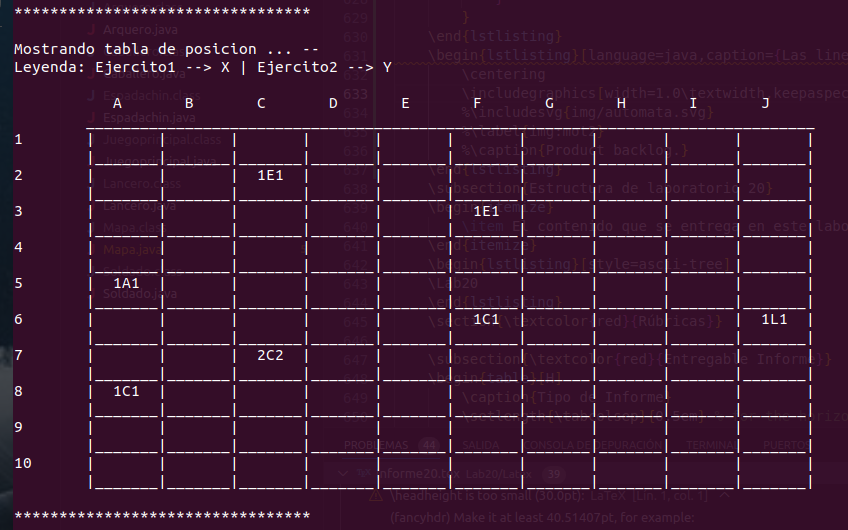
\includegraphics[width=1.0\textwidth,keepaspectratio]{img/Commit6.png}
		%\includesvg{img/automata.svg}
		%\label{img:mot2}
		%\caption{Product backlog.}
	\end{figure}
	\subsection{Ejercicio Mapa}
	\begin{itemize}	
		\item En el septimo commit creamos las funcion viewSoldiers() y bonificacion() los cuales bonficacion me permite aumentar 1 punto de vida a cada soldado de cada ejercito con 1 para cada tipo de territorio y tambien en viewSoldiers podemos ver la informacion de los soldados de cada ejercito.	
		\item El codigo y el commit seria el siguiente:
	\end{itemize}	
	\begin{lstlisting}[language=bash,caption={Commit}][H]
		$ git commit -m "Agregando a mapa las funciones como viewSoldiers() y bonificacion() los cuales nos van poder mostrar el territorio y la informacion de cada soldado la cual fue cambiada por el tipo de territorio y reino que es este ejercito"
	\end{lstlisting}	
	\begin{lstlisting}[language=java,caption={Las lineas de codigos de la clase Mapa creada:}][H]
		public void bonificacion(ArrayList<ArrayList<Soldado>> army, String territory , String kingdom) {
			for(int i = 0; i < 10; i++){ //ITERACION
				for(int j = 0; j < 10 ; j++){//ITERACION
					if(army.get(i).get(j) != null){
						if(kingdom.equals("Inglaterra") && territory.equals("bosque")){
							army.get(i).get(j).setLifeLevel(army.get(i).get(j).getLifeLevel() + 1);
						}else if(kingdom.equals("Francia") && territory.equals("campo abierto")){
							army.get(i).get(j).setLifeLevel(army.get(i).get(j).getLifeLevel() + 1);
						}else if((kingdom.equals("Castilla") || kingdom.equals("Aragon")) && territory.equals("montana")){
							army.get(i).get(j).setLifeLevel(army.get(i).get(j).getLifeLevel() + 1);
						}else if(kingdom.equals("Moros") && territory.equals("desierto")){
							army.get(i).get(j).setLifeLevel(army.get(i).get(j).getLifeLevel() + 1);
						}else if(kingdom.equals("Sacro") && (territory.equals("desierto") || territory.equals("playa") || territory.equals("campo abierto"))){
							army.get(i).get(j).setLifeLevel(army.get(i).get(j).getLifeLevel() + 1);
						}
					}
				}
			}
		} 
		public static void viewSoldiers(String armyespe, int num, ArrayList<ArrayList<Soldado>> army){
			int numbersoldiers = 0;
			System.out.println("El Ejercito " + armyespe + " del " + num + " ejercito sus soldados son :");
			for(int i = 0; i < 10; i++){ //ITERACION
				for(int j = 0; j < 10 ; j++){//ITERACION
					if(army.get(i).get(j) != null){
						System.out.println("\n*********************************");
						System.out.println("El " + (numbersoldiers + 1) + " soldado es: ");
						System.out.println(army.get(i).get(j).toString());
						numbersoldiers++;
					}
				}
			}
		}
	\end{lstlisting}
	\begin{lstlisting}[language=bash,caption={Ejecucion:}][H]
		-------------------------------------------
		--                 MENU                  --
		-------------------------------------------
		 SELECCIONE UN NUMERO PARA PODER EMPEZAR O TERMINAR
		 1 : JUGAR
		 2 : NO JUGAR
		1
		El Ejercito Francia tiene 6 soldados : 
		
		Registrando al 1 soldado del Ejercito Francia
		
		Nombre: Espadachin0X1
		Vida: 9
		Fila: 6
		Columna: H
		Nivel de ataque: 10
		Nivel de Defensa: 8
		Nivel de vida: 9
		Velocidad: 1
		Actitud: Espadachin
		Estado: true
		---------------------------------
		Registrando al 2 soldado del Ejercito Francia
		
		Nombre: Espadachin1X1
		Vida: 8
		Fila: 5
		Columna: F
		Nivel de ataque: 10
		Nivel de Defensa: 8
		Nivel de vida: 8
		Velocidad: 2
		Actitud: Espadachin
		Estado: true
		---------------------------------
		Registrando al 3 soldado del Ejercito Francia
		
		Nombre: Espadachin2X1
		Vida: 8
		Fila: 2
		Columna: G
		Nivel de ataque: 10
		Nivel de Defensa: 8
		Nivel de vida: 8
		Velocidad: 1
		Actitud: Espadachin
		Estado: true
		---------------------------------
		Registrando al 4 soldado del Ejercito Francia
		
		Nombre: Lancero3X1
		Vida: 5
		Fila: 5
		Columna: I
		Nivel de ataque: 5
		Nivel de Defensa: 10
		Nivel de vida: 5
		Velocidad: 3
		Actitud: Lancero
		Estado: true
		---------------------------------
		Registrando al 5 soldado del Ejercito Francia
		
		Nombre: Arquero4X1
		Vida: 5
		Fila: 8
		Columna: A
		Nivel de ataque: 7
		Nivel de Defensa: 3
		Nivel de vida: 5
		Velocidad: 1
		Actitud: Arquero
		Estado: true
		---------------------------------
		Registrando al 6 soldado del Ejercito Francia
		
		Nombre: Arquero5X1
		Vida: 4
		Fila: 2
		Columna: C
		Nivel de ataque: 7
		Nivel de Defensa: 3
		Nivel de vida: 4
		Velocidad: 5
		Actitud: Arquero
		Estado: true
		---------------------------------
		*********************************
		El Ejercito Castilla tiene 5 soldados : 
		
		Registrando al 1 soldado del Ejercito Castilla
		
		Nombre: Lancero0X2
		Vida: 5
		Fila: 6
		Columna: E
		Nivel de ataque: 5
		Nivel de Defensa: 10
		Nivel de vida: 5
		Velocidad: 2
		Actitud: Lancero
		Estado: true
		---------------------------------
		Registrando al 2 soldado del Ejercito Castilla
		
		Nombre: Caballero1X2
		Vida: 10
		Fila: 4
		Columna: D
		Nivel de ataque: 13
		Nivel de Defensa: 7
		Nivel de vida: 10
		Velocidad: 3
		Actitud: Caballero
		Estado: true
		---------------------------------
		Registrando al 3 soldado del Ejercito Castilla
		
		Nombre: Arquero2X2
		Vida: 5
		Fila: 7
		Columna: B
		Nivel de ataque: 7
		Nivel de Defensa: 3
		Nivel de vida: 5
		Velocidad: 1
		Actitud: Arquero
		Estado: true
		---------------------------------
		Registrando al 4 soldado del Ejercito Castilla
		
		Nombre: Espadachin3X2
		Vida: 9
		Fila: 8
		Columna: H
		Nivel de ataque: 10
		Nivel de Defensa: 8
		Nivel de vida: 9
		Velocidad: 1
		Actitud: Espadachin
		Estado: true
		---------------------------------
		Registrando al 5 soldado del Ejercito Castilla
		
		Nombre: Lancero4X2
		Vida: 7
		Fila: 4
		Columna: C
		Nivel de ataque: 5
		Nivel de Defensa: 10
		Nivel de vida: 7
		Velocidad: 1
		Actitud: Lancero
		Estado: true
		---------------------------------
		*********************************
		
		*********************************
		El tipo de territorio es: campo abierto
		
		*********************************
		El Ejercito Francia del 1 ejercito sus soldados son :
		
		*********************************
		El 1 soldado es: 
		
		Nombre: Arquero5X1
		Vida: 4
		Fila: 2
		Columna: C
		Nivel de ataque: 7
		Nivel de Defensa: 3
		Nivel de vida: 5
		Velocidad: 5
		Actitud: Arquero
		Estado: true
		
		*********************************
		El 2 soldado es: 
		
		Nombre: Espadachin2X1
		Vida: 8
		Fila: 2
		Columna: G
		Nivel de ataque: 10
		Nivel de Defensa: 8
		Nivel de vida: 9
		Velocidad: 1
		Actitud: Espadachin
		Estado: true
		
		*********************************
		El 3 soldado es: 
		
		Nombre: Espadachin1X1
		Vida: 8
		Fila: 5
		Columna: F
		Nivel de ataque: 10
		Nivel de Defensa: 8
		Nivel de vida: 9
		Velocidad: 2
		Actitud: Espadachin
		Estado: true
		
		*********************************
		El 4 soldado es: 
		
		Nombre: Lancero3X1
		Vida: 5
		Fila: 5
		Columna: I
		Nivel de ataque: 5
		Nivel de Defensa: 10
		Nivel de vida: 6
		Velocidad: 3
		Actitud: Lancero
		Estado: true
		
		*********************************
		El 5 soldado es: 
		
		Nombre: Espadachin0X1
		Vida: 9
		Fila: 6
		Columna: H
		Nivel de ataque: 10
		Nivel de Defensa: 8
		Nivel de vida: 10
		Velocidad: 1
		Actitud: Espadachin
		Estado: true
		
		*********************************
		El 6 soldado es: 
		
		Nombre: Arquero4X1
		Vida: 5
		Fila: 8
		Columna: A
		Nivel de ataque: 7
		Nivel de Defensa: 3
		Nivel de vida: 6
		Velocidad: 1
		Actitud: Arquero
		Estado: true
		El Ejercito Castilla del 2 ejercito sus soldados son :
		
		*********************************
		El 1 soldado es: 
		
		Nombre: Lancero4X2
		Vida: 7
		Fila: 4
		Columna: C
		Nivel de ataque: 5
		Nivel de Defensa: 10
		Nivel de vida: 7
		Velocidad: 1
		Actitud: Lancero
		Estado: true
		
		*********************************
		El 2 soldado es: 
		
		Nombre: Caballero1X2
		Vida: 10
		Fila: 4
		Columna: D
		Nivel de ataque: 13
		Nivel de Defensa: 7
		Nivel de vida: 10
		Velocidad: 3
		Actitud: Caballero
		Estado: true
		
		*********************************
		El 3 soldado es: 
		
		Nombre: Lancero0X2
		Vida: 5
		Fila: 6
		Columna: E
		Nivel de ataque: 5
		Nivel de Defensa: 10
		Nivel de vida: 5
		Velocidad: 2
		Actitud: Lancero
		Estado: true
		
		*********************************
		El 4 soldado es: 
		
		Nombre: Arquero2X2
		Vida: 5
		Fila: 7
		Columna: B
		Nivel de ataque: 7
		Nivel de Defensa: 3
		Nivel de vida: 5
		Velocidad: 1
		Actitud: Arquero
		Estado: true
		
		*********************************
		El 5 soldado es: 
		
		Nombre: Espadachin3X2
		Vida: 9
		Fila: 8
		Columna: H
		Nivel de ataque: 10
		Nivel de Defensa: 8
		Nivel de vida: 9
		Velocidad: 1
		Actitud: Espadachin
		Estado: true
		
		
	\end{lstlisting}
	\begin{figure}[H]
		\centering
		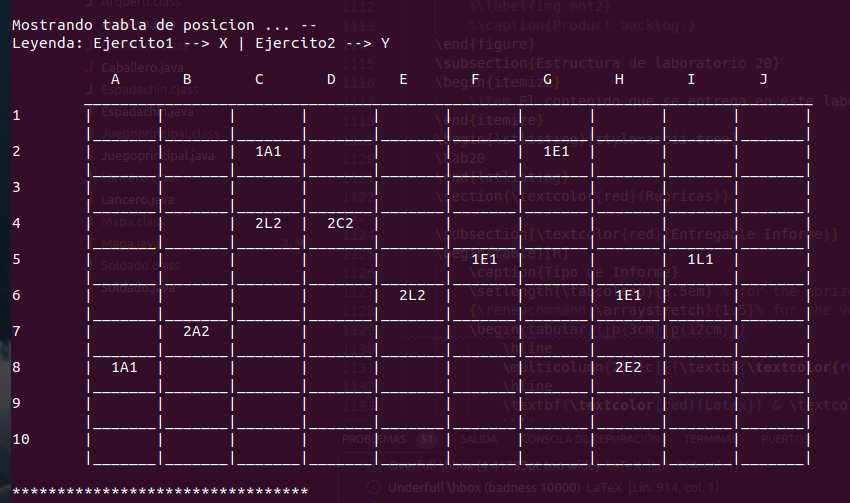
\includegraphics[width=1.0\textwidth,keepaspectratio]{img/Commit7.png}
		%\includesvg{img/automata.svg}
		%\label{img:mot2}
		%\caption{Product backlog.}
	\end{figure}
	\subsection{Ejercicio Mapa}
	\begin{itemize}	
		\item En el octavo commit creamos las funcion longerLife() el cual nos retorna especificaiones del soldado con mayor vida del ejercito;
		\item El codigo y el commit seria el siguiente:
	\end{itemize}	
	\begin{lstlisting}[language=bash,caption={Commit}][H]
		$ git commit -m "Agregando la funcion longerlife() el cual me dara al soldado con mayor vida y sus especificaciones"
	\end{lstlisting}	
	\begin{lstlisting}[language=java,caption={Las lineas de codigos de la clase Mapa creada:}][H]
		public static void longerLife(ArrayList<ArrayList<Soldado>> army, String kingdom){
			int mayor = 0;//METODO CREADO PARA PODER PERMITIRNOS A CONOCER EL SOLDADO CON MAYOR VIDA DE CADA EJERCITO 
			Soldado soldier = null;
			for(int i = 0; i < army.size(); i++){
				for(int j = 0; j < army.get(i).size(); j++){
					if(army.get(i).get(j) != null){ //COMPROBACION QUE HACEMOS PARA PODER DECIR QUE EL CASILLERO DONDE ESTAMOS ES UN SOLDADO QUE EXISTE
						if(army.get(i).get(j).getLifeActual() > mayor){ //COMPARAMOS PUNTOS DE VIDA DE CADA SOLDADO PARA VER QUIEN ES EL MAYOR 
							mayor = army.get(i).get(j).getLifeActual();
							soldier = army.get(i).get(j);
						}
					}
				}
			}
			System.out.println("El soldado con mayor vida del Ejercito " + kingdom + " es: ");
			System.out.println(soldier.toString());//IMPRIMIMOS SUS DATOS PARA PODER VER DE QUE SOLDADO SE TRATA 
			System.out.println("*********************************");
		}
	\end{lstlisting}
	\begin{lstlisting}[language=bash,caption={Ejecucion:}][H]
		-------------------------------------------
		--                 MENU                  --
		-------------------------------------------
		 SELECCIONE UN NUMERO PARA PODER EMPEZAR O TERMINAR
		 1 : JUGAR
		 2 : NO JUGAR
		1
		El Ejercito Aragon tiene 3 soldados : 
		
		Registrando al 1 soldado del Ejercito Aragon
		
		Nombre: Lancero0X1
		Vida: 6
		Fila: 6
		Columna: G
		Nivel de ataque: 5
		Nivel de Defensa: 10
		Nivel de vida: 6
		Velocidad: 1
		Actitud: Lancero
		Estado: true
		---------------------------------
		Registrando al 2 soldado del Ejercito Aragon
		
		Nombre: Espadachin1X1
		Vida: 9
		Fila: 8
		Columna: F
		Nivel de ataque: 10
		Nivel de Defensa: 8
		Nivel de vida: 9
		Velocidad: 4
		Actitud: Espadachin
		Estado: true
		---------------------------------
		Registrando al 3 soldado del Ejercito Aragon
		
		Nombre: Espadachin2X1
		Vida: 9
		Fila: 3
		Columna: E
		Nivel de ataque: 10
		Nivel de Defensa: 8
		Nivel de vida: 9
		Velocidad: 1
		Actitud: Espadachin
		Estado: true
		---------------------------------
		*********************************
		El Ejercito Inglaterra tiene 3 soldados : 
		
		Registrando al 1 soldado del Ejercito Inglaterra
		
		Nombre: Espadachin0X2
		Vida: 9
		Fila: 3
		Columna: A
		Nivel de ataque: 10
		Nivel de Defensa: 8
		Nivel de vida: 9
		Velocidad: 5
		Actitud: Espadachin
		Estado: true
		---------------------------------
		Registrando al 2 soldado del Ejercito Inglaterra
		
		Nombre: Arquero1X2
		Vida: 3
		Fila: 6
		Columna: H
		Nivel de ataque: 7
		Nivel de Defensa: 3
		Nivel de vida: 3
		Velocidad: 4
		Actitud: Arquero
		Estado: true
		---------------------------------
		Registrando al 3 soldado del Ejercito Inglaterra
		
		Nombre: Caballero2X2
		Vida: 12
		Fila: 7
		Columna: I
		Nivel de ataque: 13
		Nivel de Defensa: 7
		Nivel de vida: 12
		Velocidad: 1
		Actitud: Caballero
		Estado: true
		---------------------------------
		*********************************
		
		*********************************
		El tipo de territorio es: desierto
		
		*********************************
		El Ejercito Aragon del 1 ejercito sus soldados son :
		
		*********************************
		El 1 soldado es: 
		
		Nombre: Espadachin2X1
		Vida: 9
		Fila: 3
		Columna: E
		Nivel de ataque: 10
		Nivel de Defensa: 8
		Nivel de vida: 9
		Velocidad: 1
		Actitud: Espadachin
		Estado: true
		
		*********************************
		El 2 soldado es: 
		
		Nombre: Lancero0X1
		Vida: 6
		Fila: 6
		Columna: G
		Nivel de ataque: 5
		Nivel de Defensa: 10
		Nivel de vida: 6
		Velocidad: 1
		Actitud: Lancero
		Estado: true
		
		*********************************
		El 3 soldado es: 
		
		Nombre: Espadachin1X1
		Vida: 9
		Fila: 8
		Columna: F
		Nivel de ataque: 10
		Nivel de Defensa: 8
		Nivel de vida: 9
		Velocidad: 4
		Actitud: Espadachin
		Estado: true
		El Ejercito Inglaterra del 2 ejercito sus soldados son :
		
		*********************************
		El 1 soldado es: 
		
		Nombre: Espadachin0X2
		Vida: 9
		Fila: 3
		Columna: A
		Nivel de ataque: 10
		Nivel de Defensa: 8
		Nivel de vida: 9
		Velocidad: 5
		Actitud: Espadachin
		Estado: true
		
		*********************************
		El 2 soldado es: 
		
		Nombre: Arquero1X2
		Vida: 3
		Fila: 6
		Columna: H
		Nivel de ataque: 7
		Nivel de Defensa: 3
		Nivel de vida: 3
		Velocidad: 4
		Actitud: Arquero
		Estado: true
		
		*********************************
		El 3 soldado es: 
		
		Nombre: Caballero2X2
		Vida: 12
		Fila: 7
		Columna: I
		Nivel de ataque: 13
		Nivel de Defensa: 7
		Nivel de vida: 12
		Velocidad: 1
		Actitud: Caballero
		Estado: true
		
	\end{lstlisting}
	\begin{figure}[H]
		\centering
		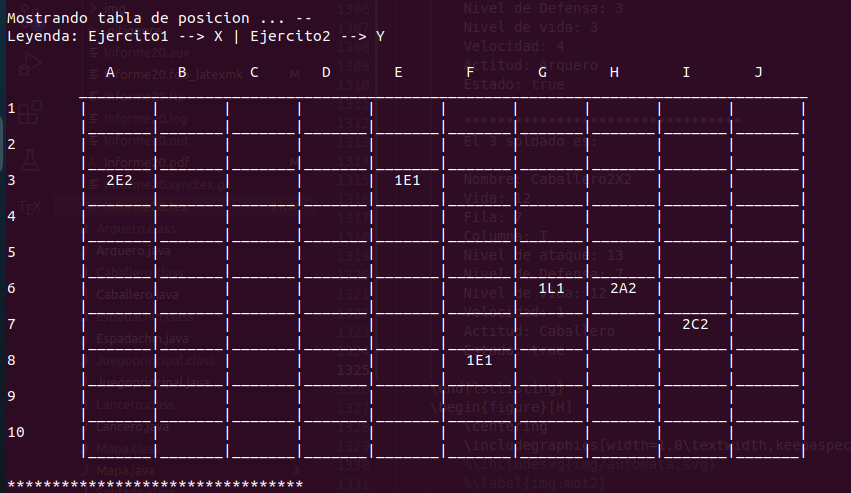
\includegraphics[width=1.0\textwidth,keepaspectratio]{img/Commit8.png}
		%\includesvg{img/automata.svg}
		%\label{img:mot2}
		%\caption{Product backlog.}
	\end{figure}
	\begin{lstlisting}[language=bash,caption={Ejecucion:}][H]
		*********************************
		El soldado con mayor vida del Ejercito Aragon es: 
		
		Nombre: Espadachin2X1
		Vida: 9
		Fila: 3
		Columna: E
		Nivel de ataque: 10
		Nivel de Defensa: 8
		Nivel de vida: 9
		Velocidad: 1
		Actitud: Espadachin
		Estado: true
		*********************************
		El soldado con mayor vida del Ejercito Inglaterra es: 
		
		Nombre: Caballero2X2
		Vida: 12
		Fila: 7
		Columna: I
		Nivel de ataque: 13
		Nivel de Defensa: 7
		Nivel de vida: 12
		Velocidad: 1
		Actitud: Caballero
		Estado: true
		*********************************
	\end{lstlisting}
	\subsection{Estructura de laboratorio 20}
	\begin{itemize}	
		\item El contenido que se entrega en este laboratorio20 es el siguiente:
	\end{itemize}
	\begin{lstlisting}[style=ascii-tree]
	\Lab20
	\end{lstlisting}    
	\section{\textcolor{red}{Rúbricas}}
	
	\subsection{\textcolor{red}{Entregable Informe}}
	\begin{table}[H]
		\caption{Tipo de Informe}
		\setlength{\tabcolsep}{0.5em} % for the horizontal padding
		{\renewcommand{\arraystretch}{1.5}% for the vertical padding
		\begin{tabular}{|p{3cm}|p{12cm}|}
			\hline
			\multicolumn{2}{|c|}{\textbf{\textcolor{red}{Informe}}}  \\
			\hline 
			\textbf{\textcolor{red}{Latex}} & \textcolor{blue}{El informe está en formato PDF desde Latex,  con un formato limpio (buena presentación) y facil de leer.}   \\ 
			\hline 
			
			
		\end{tabular}
	}
	\end{table}
	
	\clearpage
	
	\subsection{\textcolor{red}{Rúbrica para el contenido del Informe y demostración}}
	\begin{itemize}			
		\item El alumno debe marcar o dejar en blanco en celdas de la columna \textbf{Checklist} si cumplio con el ítem correspondiente.
		\item Si un alumno supera la fecha de entrega,  su calificación será sobre la nota mínima aprobada, siempre y cuando cumpla con todos lo items.
		\item El alumno debe autocalificarse en la columna \textbf{Estudiante} de acuerdo a la siguiente tabla:
	
		\begin{table}[ht]
			\caption{Niveles de desempeño}
			\begin{center}
			\begin{tabular}{ccccc}
    			\hline
    			 & \multicolumn{4}{c}{Nivel}\\
    			\cline{1-5}
    			\textbf{Puntos} & Insatisfactorio 25\%& En Proceso 50\% & Satisfactorio 75\% & Sobresaliente 100\%\\
    			\textbf{2.0}&0.5&1.0&1.5&2.0\\
    			\textbf{4.0}&1.0&2.0&3.0&4.0\\
    		\hline
			\end{tabular}
		\end{center}
	\end{table}	
	
	\end{itemize}
	
	\begin{table}[H]
		\caption{Rúbrica para contenido del Informe y demostración}
		\setlength{\tabcolsep}{0.5em} % for the horizontal padding
		{\renewcommand{\arraystretch}{1.5}% for the vertical padding
		%\begin{center}
		\begin{tabular}{|p{2.7cm}|p{7cm}|x{1.3cm}|p{1.2cm}|p{1.5cm}|p{1.1cm}|}
			\hline
    		\multicolumn{2}{|c|}{Contenido y demostración} & Puntos & Checklist & Estudiante & Profesor\\
			\hline
			\textbf{1. GitHub} & Hay enlace URL activo del directorio para el  laboratorio hacia su repositorio GitHub con código fuente terminado y fácil de revisar. &2 &X &2 & \\ 
			\hline
			\textbf{2. Commits} &  Hay capturas de pantalla de los commits más importantes con sus explicaciones detalladas. (El profesor puede preguntar para refrendar calificación). &4 &X &4 & \\ 
			\hline 
			\textbf{3. Código fuente} &  Hay porciones de código fuente importantes con numeración y explicaciones detalladas de sus funciones. &2 &X &2 & \\ 
			\hline 
			\textbf{4. Ejecución} & Se incluyen ejecuciones/pruebas del código fuente  explicadas gradualmente. &2 &X &2 & \\ 
			\hline			
			\textbf{5. Pregunta} & Se responde con completitud a la pregunta formulada en la tarea.  (El profesor puede preguntar para refrendar calificación).  &2 &X &2 & \\ 
			\hline	
			\textbf{6. Fechas} & Las fechas de modificación del código fuente estan dentro de los plazos de fecha de entrega establecidos. &2 &X &2 & \\ 
			\hline 
			\textbf{7. Ortografía} & El documento no muestra errores ortográficos. &2 &X &2 & \\ 
			\hline 
			\textbf{8. Madurez} & El Informe muestra de manera general una evolución de la madurez del código fuente,  explicaciones puntuales pero precisas y un acabado impecable.   (El profesor puede preguntar para refrendar calificación).  &4 &X &2 & \\ 
			\hline
			\multicolumn{2}{|c|}{\textbf{Total}} &20 & &18 & \\ 
			\hline
		\end{tabular}
		%\end{center}
		%\label{tab:multicol}
		}
	\end{table}
	
\clearpage

\section{Referencias}
\begin{itemize}			
	\item \url{https://drive.google.com/drive/u/1/folders/19TzLFO-T77qG7bOWmg5OH7FXAMD2CrJL}
\end{itemize}	
	
%\clearpage
%\bibliographystyle{apalike}
%\bibliographystyle{IEEEtranN}
%\bibliography{bibliography}
			
\end{document}